% Dit werk is gelicenseerd onder de licentie Creative Commons Naamsvermelding-GelijkDelen 4.0 Internationaal. Ga naar http://creativecommons.org/licenses/by-sa/4.0/ om een kopie van de licentie te kunnen lezen.
\documentclass[t]{beamer}

%%%%%%%%%%%%%%%%%%%%%%%%%%%%%%
% Packages
%%%%%%%%%%%%%%%%%%%%%%%%%%%%%%

\usepackage[dutch]{babel}               % Voor nederlandstalige hyphenatie (woordsplitsing)
\uselanguage{dutch}
\languagepath{dutch}
\usepackage{url}                        % Om url's te verwerken
\usepackage{graphicx,subfigure}         % Om figuren te kunnen verwerken
\usepackage[utf8]{inputenc}             % Om niet ascii karakters rechtstreeks te kunnen typen
\usepackage{multicol}
\usepackage[absolute,overlay]{textpos}

%%%%%%%%%%%%%%%%%%%%%%%%%%%%%%
% Layout
%%%%%%%%%%%%%%%%%%%%%%%%%%%%%%
\usetheme{Frankfurt}
\usefonttheme[onlymath]{serif}
\setbeamertemplate{footline}[page number]
\AtBeginSection[]
{
  \begin{frame}
    \frametitle{Inhoud}
    \tableofcontents[currentsection]
  \end{frame}
}

\setbeamertemplate{navigation symbols}{}

%%%%%%%%%%%%%%%%%%%%%%%%%%%%%%
% Title
%%%%%%%%%%%%%%%%%%%%%%%%%%%%%%
\title{Inleiding tot Inkscape}
\author{Brecht Baeten\inst{1}}
\institute{
	\inst{1}%
  		e-mail: brecht.baeten@gmail.com
}
\date{\today}
%%%%%%%%%%%%%%%%%%%%%%%%%%%%%%
% Omgevingen
%%%%%%%%%%%%%%%%%%%%%%%%%%%%%%

\begin{document}
	\frame{\titlepage}
%%%%%%%%%%%%%%%%%%%%%%%%%%%%%%%%%%%%%%%%%%%%%%%%%%%%%%%%%%%%%%%%%%%%%%%%%%%%%%%%
	\section{Vector graphics}
%%%%%%%%%%%%%%%%%%%%%%%%%%%%%%%%%%%%%%%%%%%%%%%%%%%%%%%%%%%%%%%%%%%%%%%%%%%%%%%%
	\begin{frame}
		\frametitle{Bitmap vs. Vector}
		\vspace{0.5cm}
		\begin{columns}
			\begin{column}[T]{0.5\textwidth}
				\includegraphics[width=\textwidth]{fig/logo_zoom_png}
				\vspace{0.5cm}
				.bmp, .png, .jpg,...
			\end{column}
			\begin{column}[T]{0.5\textwidth}
				\includegraphics[width=\textwidth]{fig/logo_zoom_pdf}
				\vspace{0.5cm}
				.svg, .eps, .cdr, .ai, .pdf,...
			\end{column}
		\end{columns}
	\end{frame}
%%%%%%%%%%%%%%%%%%%%%%%%%%%%%%%%%%%%%%%%%%%%%%%%%%%%%%%%%%%%%%%%%%%%%%%%%%%%%%%%
	\begin{frame}
		\frametitle{Scalable Vector Graphics}
		\begin{itemize}
			\item .svg
			\item W3C norm (zoals html, css, xml,...)
			\item "leesbare" bestanden
			\item "definitie" van de tekening
		\end{itemize}
		\vspace{0.5cm}
		\begin{center}
			\hfill 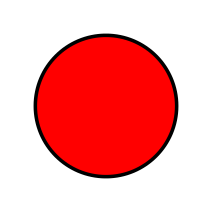
\includegraphics[width=0.2\textwidth]{fig/simpele_tekening}\\
			\vspace{-0.2cm}
			\includegraphics[width=\textwidth]{fig/simpele_tekening_bron.png}
		\end{center}	
	\end{frame}
%%%%%%%%%%%%%%%%%%%%%%%%%%%%%%%%%%%%%%%%%%%%%%%%%%%%%%%%%%%%%%%%%%%%%%%%%%%%%%%%
	\section{Inkscape}
%%%%%%%%%%%%%%%%%%%%%%%%%%%%%%%%%%%%%%%%%%%%%%%%%%%%%%%%%%%%%%%%%%%%%%%%%%%%%%%%
	\begin{frame}
		\frametitle{Werkbalken}
		\begin{center}
			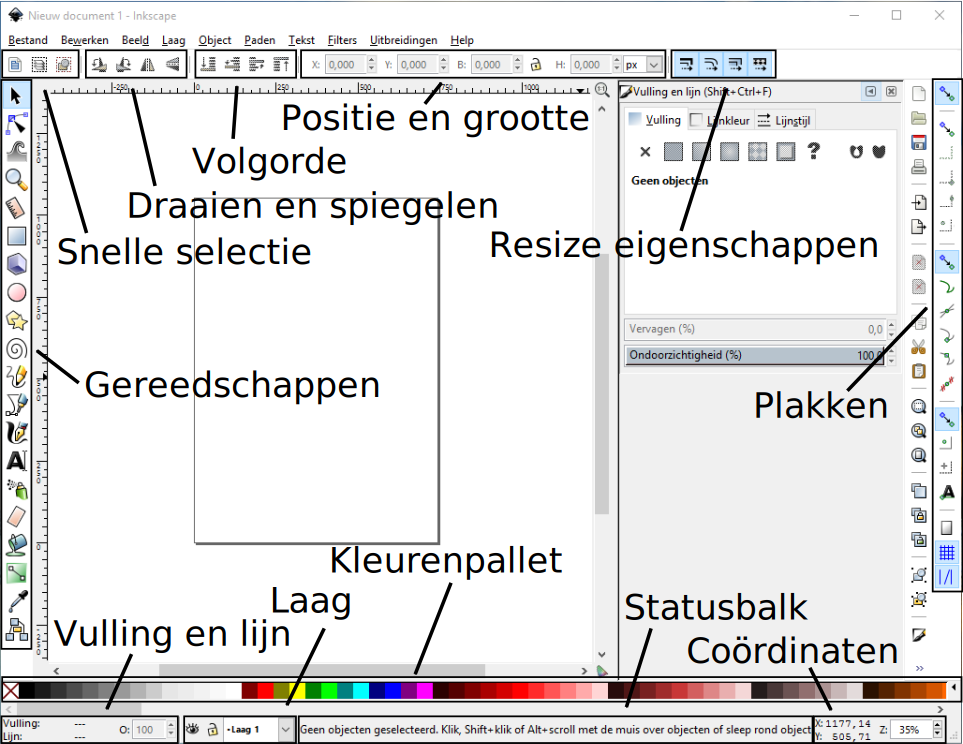
\includegraphics[height=0.85\textheight]{fig/inkscape_werkbalken}\\
		\end{center}	
	\end{frame}
%%%%%%%%%%%%%%%%%%%%%%%%%%%%%%%%%%%%%%%%%%%%%%%%%%%%%%%%%%%%%%%%%%%%%%%%%%%%%%%%
	\section{Objecten en Paden}
%%%%%%%%%%%%%%%%%%%%%%%%%%%%%%%%%%%%%%%%%%%%%%%%%%%%%%%%%%%%%%%%%%%%%%%%%%%%%%%%
	\begin{frame}
		\frametitle{Objecten}
		\begin{columns}
			\begin{column}[T]{0.6\textwidth}
				\begin{itemize}
					\item Rechthoek / 3D doos / Cirkel / Veelhoek / ster / Spiraal / Tekst
					\item Gereedschap selecteren en slepen
				\end{itemize}
				\begin{itemize}
					\item Vulling en lijn pallet openen via \emph{Object $>$ Vulling en lijn...}\\
					 of \textbf{Ctrl} + \textbf{Shift} + F\\
					 of dubbelklikken op vulling en lijn detail (links onderaan)
					\item Vulling kleur, Lijnkleur, Lijndikte, Lijnstijl
				\end{itemize}
			\end{column}
			\begin{column}[T]{0.4\textwidth}
				\includegraphics[height=0.8\textheight]{fig/inkscape_objecten}
			\end{column}
		\end{columns}
	\end{frame}
%%%%%%%%%%%%%%%%%%%%%%%%%%%%%%%%%%%%%%%%%%%%%%%%%%%%%%%%%%%%%%%%%%%%%%%%%%%%%%%%
	\begin{frame}
		\frametitle{Objecten en kleuren}
		\only<1>{
			\textbf{Tips:}
			\begin{itemize}
				\item kleurenpallet klik = vulling kleur
				\item \textbf{Shift} + kleurenpallet klik  = rand kleur
			\end{itemize}
		}
		\only<2>{
			\begin{center}
				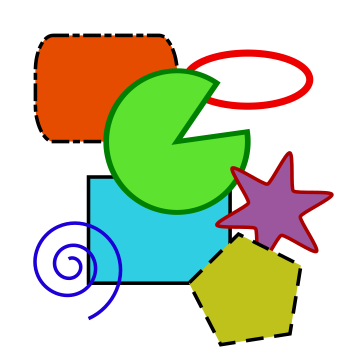
\includegraphics[height=0.8\textheight]{fig/objecten_en_kleuren}
			\end{center}
		}
	\end{frame}
%%%%%%%%%%%%%%%%%%%%%%%%%%%%%%%%%%%%%%%%%%%%%%%%%%%%%%%%%%%%%%%%%%%%%%%%%%%%%%%%
	\begin{frame}
		\frametitle{Objecten selecteren, verplaatsen en dupliceren}
		\only<1>{
			\begin{columns}
				\begin{column}[T]{0.6\textwidth}
					\begin{itemize}
						\item Selectie gereedschap
						\item Aanklikken of volledig rond slepen om een object te selecteren
					\end{itemize}
					\begin{itemize}
						\item Object selecteren en slepen om te verplaatsen
					\end{itemize}
					\begin{itemize}
						\item \emph{Bewerken $>$ Dupliceren}
					\end{itemize}
				\end{column}
				\begin{column}[T]{0.4\textwidth}
					\includegraphics[height=0.8\textheight]{fig/inkscape_selectie_gereedschap}
				\end{column}
			\end{columns}
		}
		\only<2>{
			\textbf{Tips:}
			\begin{itemize}
				\item \textbf{Ctrl} + D = dupliceren
				\item \textbf{Ctrl} + slepen = horizontaal of verticaal slepen
				\item slepen + \textbf{spatie} = object dupliceren en plaatsen (stempelen)
			\end{itemize}
		}
	\end{frame}
%%%%%%%%%%%%%%%%%%%%%%%%%%%%%%%%%%%%%%%%%%%%%%%%%%%%%%%%%%%%%%%%%%%%%%%%%%%%%%%%
	\begin{frame}
		\frametitle{Objecten draaien en transformeren}
		\only<1>{
			\begin{columns}
				\begin{column}[T]{0.6\textwidth}
					\begin{itemize}
						\item Selecteren om te: 
						\item Vergroten / Verkleinen
					\end{itemize}
					\begin{itemize}
						\item nog eens klikken om te:
						\item Draaien
						\item Scheeftrekken
						\item Verplaatsbaar referentiepunt
					\end{itemize}
					\begin{itemize}
						\item Ieder object heeft zijn eigen specifieke vervormings eigenschappen, beschikbaar via het object gereedschap
					\end{itemize}
				\end{column}
				\begin{column}[T]{0.4\textwidth}
					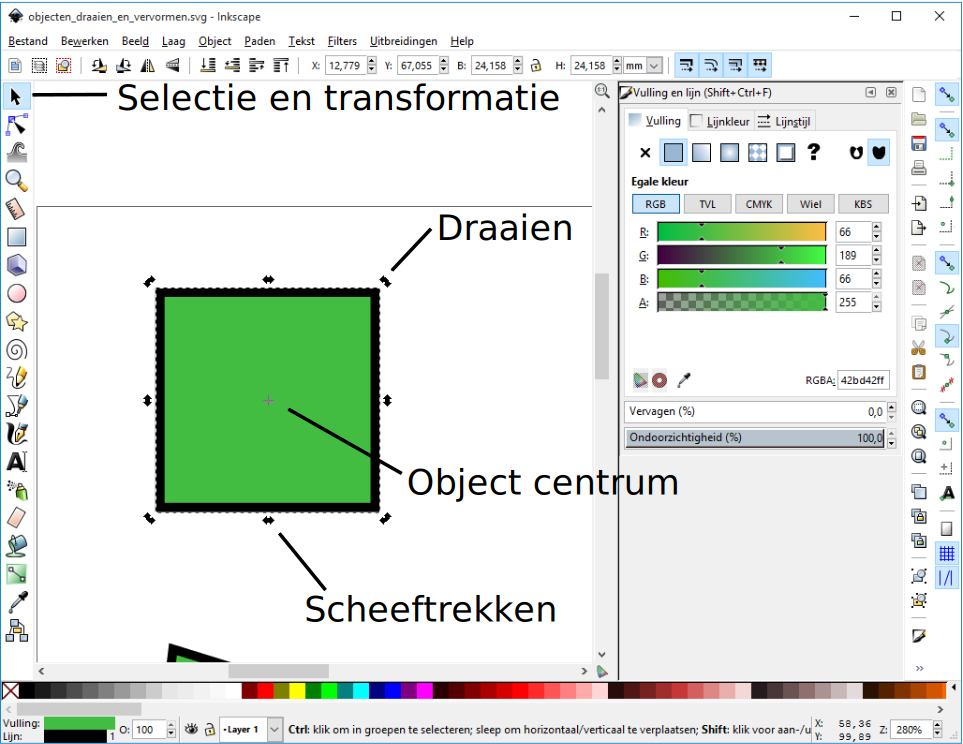
\includegraphics[height=0.8\textheight]{fig/inkscape_objecten_draaien_en_transformeren}
				\end{column}
			\end{columns}
		}
		\only<2>{
			\begin{center}
				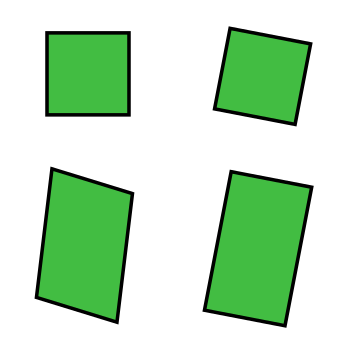
\includegraphics[height=0.8\textheight]{fig/objecten_draaien_en_transformeren}
			\end{center}	
		}
		\only<3>{
			\textbf{Tips:}
			\begin{itemize}
				\item \textbf{Ctrl} + vervormen = behoud van aspect ratio
				\item \textbf{Shift} + vervormen = schalen rond referentiepunt
				\item \textbf{Ctrl} + \textbf{Shift} + vervormen = combinatie van bovenstaande
				\item \textbf{Ctrl} + draaien = draaien met stappen van 15$^\circ$
			\end{itemize}
		}	
	\end{frame}
%%%%%%%%%%%%%%%%%%%%%%%%%%%%%%%%%%%%%%%%%%%%%%%%%%%%%%%%%%%%%%%%%%%%%%%%%%%%%%%%
	\begin{frame}
		\frametitle{Objecten groeperen en volgorde}
		\only<1>{
			\begin{columns}
				\begin{column}[T]{0.6\textwidth}
					\begin{itemize}
						\item Meerdere objecten selecteren met \textbf{Shift} + klik of door een kader errond te slepen
						\item Groeperen / groep opheffen
					\end{itemize}
					\begin{itemize}
						\item Gegroepeerde objecten gedragen zich als één object
						\item Schalen
						\item Roteren
						\item Scheeftrekken
					\end{itemize}
					\begin{itemize}
						\item Volgorde van overlappende objecten aanpassen met \textbf{PageUp} \textbf{PageDown}
					\end{itemize}
				\end{column}
				\begin{column}[T]{0.4\textwidth}
					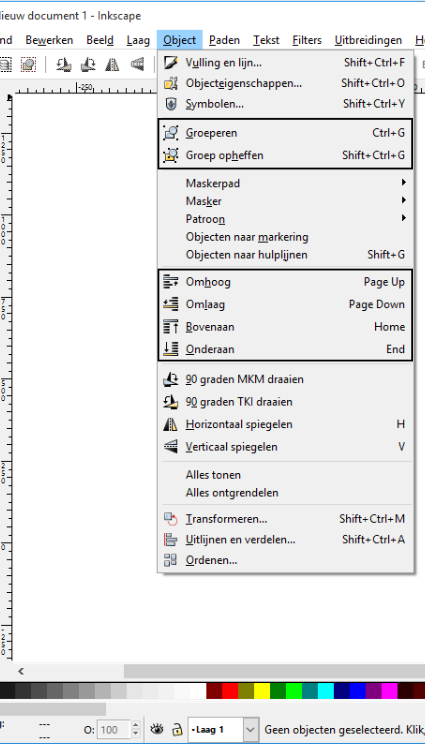
\includegraphics[height=0.8\textheight]{fig/inkscape_objecten_groeperen}
				\end{column}
			\end{columns}
		}
		\only<2>{
			\textbf{Tips:}
			\begin{itemize}
				\item \textbf{Ctrl} + G = Groeperen
				\item \textbf{Ctrl} + \textbf{Shift} + G = Groep opheffen
				\item Dubbelklikken op een groep is de groep bewerken
				\item \textbf{Ctrl} + klikken = één object uit een groep selecteren om te bewerken
				\item \textbf{Alt} + klikken = onderliggende objecten selecteren
			\end{itemize}
		}
	\end{frame}
%%%%%%%%%%%%%%%%%%%%%%%%%%%%%%%%%%%%%%%%%%%%%%%%%%%%%%%%%%%%%%%%%%%%%%%%%%%%%%%%
	\begin{frame}
		\frametitle{Objecten vs. Paden}
		
		\vspace{-0.5cm}
		\hfill 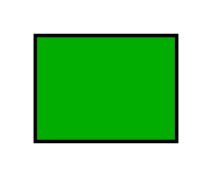
\includegraphics[width=0.2\textwidth]{fig/rechthoek_object}\\
		\vspace{-0.3cm}
		\includegraphics[height=2.5cm]{fig/rechthoek_object_bron.png}
		
		\hfill \includegraphics[width=0.2\textwidth]{fig/rechthoek_pad}\\
		\vspace{-0.3cm}
		\includegraphics[height=2.5cm]{fig/rechthoek_pad_bron.png}	
	\end{frame}
%%%%%%%%%%%%%%%%%%%%%%%%%%%%%%%%%%%%%%%%%%%%%%%%%%%%%%%%%%%%%%%%%%%%%%%%%%%%%%%%
	\begin{frame}
		\frametitle{Paden}	
		\only<1>{
			\begin{columns}
				\begin{column}[T]{0.6\textwidth}
					\begin{itemize}
						\item Losse hand tekenen
						\item Rechten / Bezier krommen / Splines
					\end{itemize}
					\begin{itemize}
						\item Van punt tot punt klikken voor een gebroken lijn
						\item Klikken en slepen voor een vloeiende lijn
						\item Dubbelklik om te eindigen
						\item Rechter muis klik om bij het vorige punt te stoppen
					\end{itemize}
				\end{column}
				\begin{column}[T]{0.4\textwidth}
					\includegraphics[height=0.8\textheight]{fig/inkscape_paden}
				\end{column}
			\end{columns}
		}
		\only<2>{
			\begin{columns}
				\begin{column}[T]{0.6\textwidth}
					\begin{itemize}
						\item Pad bewerken gereedschap
					\end{itemize}
					\begin{itemize}
						\item Knopen toevoegen / verwijderen
						\item Knopen samenvoegen / uiteen halen
						\item Knopen verbinden met een lijn
						\item Lijn tussen Knopen verwijderen
					\end{itemize}
					\begin{itemize}
						\item Knooppunt type\\ (hoekig/glad/symmetrisch/auto)
					\end{itemize}
					\begin{itemize}
						\item Lijn vs. Curve
						\item Object naar pad
						\item Lijn (met dikte) naar pad
					\end{itemize}
				\end{column}
				\begin{column}[T]{0.4\textwidth}
					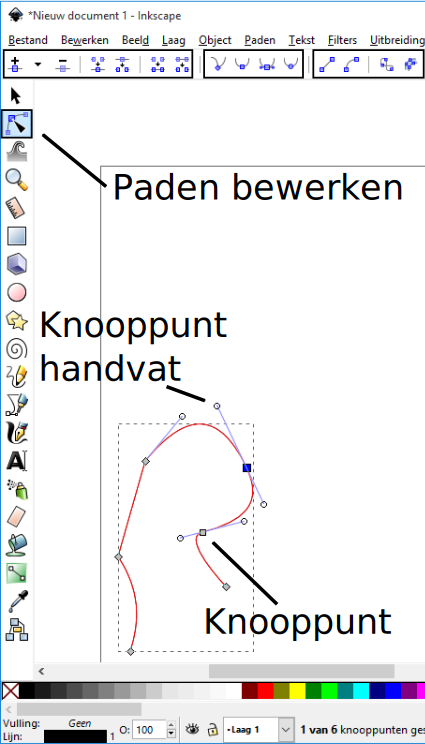
\includegraphics[height=0.8\textheight]{fig/inkscape_paden_bewerken}
				\end{column}
			\end{columns}
		}
		\only<3>{
			\begin{center}
				
\includegraphics[height=0.8\textheight]{fig/paden}
			\end{center}
		}
	\end{frame}
%%%%%%%%%%%%%%%%%%%%%%%%%%%%%%%%%%%%%%%%%%%%%%%%%%%%%%%%%%%%%%%%%%%%%%%%%%%%%%%%
	\begin{frame}
		\frametitle{Pad operaties}
		\only<1>{
			\begin{columns}
				\begin{column}[T]{0.6\textwidth}
					\begin{itemize}
						\item Elementaire bewerkingen op paden
					\end{itemize}
					\begin{itemize}
						\item Vereniging
						\item Verschil
						\item Overlap
						\item Uitsluiting
						\item Splitsing
						\item Snijden
					\end{itemize}
				\end{column}
				\begin{column}[T]{0.4\textwidth}
					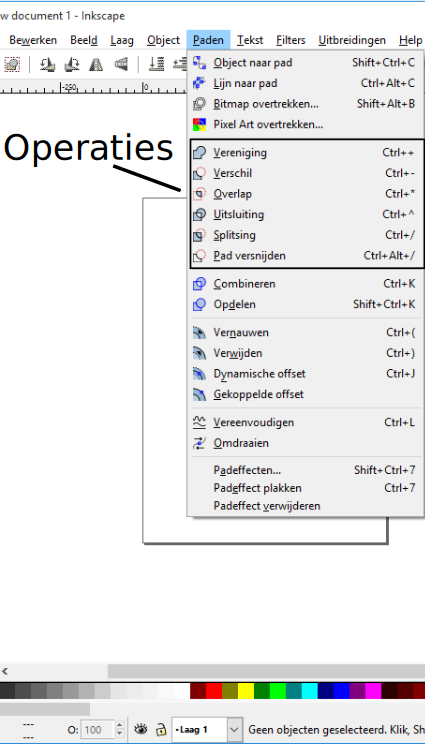
\includegraphics[height=0.8\textheight]{fig/inkscape_pad_operaties}
				\end{column}
			\end{columns}
		}
		\only<2>{
			\begin{center}
				
\includegraphics[height=0.8\textheight]{fig/pad_operaties}
			\end{center}
		}
	\end{frame}	
%%%%%%%%%%%%%%%%%%%%%%%%%%%%%%%%%%%%%%%%%%%%%%%%%%%%%%%%%%%%%%%%%%%%%%%%%%%%%%%%
	\section{Document eigenschappen}
%%%%%%%%%%%%%%%%%%%%%%%%%%%%%%%%%%%%%%%%%%%%%%%%%%%%%%%%%%%%%%%%%%%%%%%%%%%%%%%%
	\begin{frame}
		\frametitle{Pagina afmetingen}
		\begin{center}
			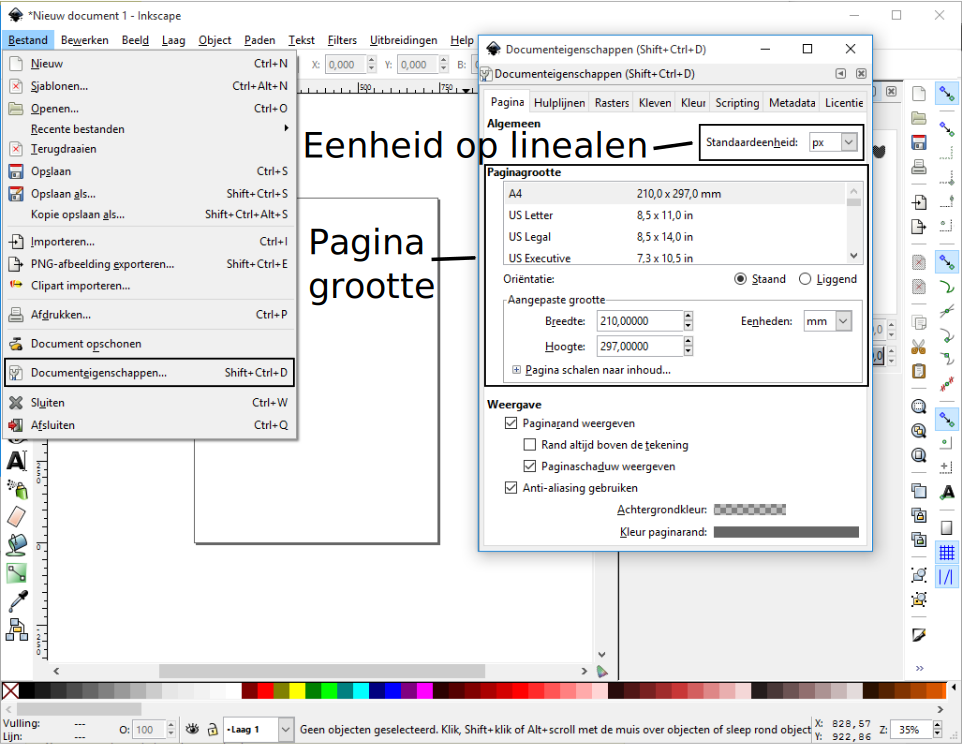
\includegraphics[height=0.8\textheight]{fig/inkscape_documenteigenschappen}
		\end{center}	
	\end{frame}
%%%%%%%%%%%%%%%%%%%%%%%%%%%%%%%%%%%%%%%%%%%%%%%%%%%%%%%%%%%%%%%%%%%%%%%%%%%%%%%%
	\begin{frame}
		\frametitle{Sjablonen}
			\begin{columns}
				\begin{column}[T]{0.6\textwidth}
					\begin{itemize}
						\item Verschillende paginagroottes, standaard eenheden, linealen,...
					\end{itemize}
					\begin{itemize}
						\item Zelf templates opslaan in\\ \emph{'inkscape dir'/share/templates/}
						\item Wanneer inkscape start wordt \emph{default.svg} of \emph{default.nl.svg} geladen
					\end{itemize}
					
					\vspace{1cm}
					Maak een A4 document met eenheden in mm en gebruik dit als default.
				\end{column}
				\begin{column}[T]{0.4\textwidth}
					\includegraphics[height=0.8\textheight]{fig/inkscape_sjablonen}
				\end{column}
			\end{columns}
	\end{frame}
%%%%%%%%%%%%%%%%%%%%%%%%%%%%%%%%%%%%%%%%%%%%%%%%%%%%%%%%%%%%%%%%%%%%%%%%%%%%%%%%	
	\section{Rasters en hulplijnen}
%%%%%%%%%%%%%%%%%%%%%%%%%%%%%%%%%%%%%%%%%%%%%%%%%%%%%%%%%%%%%%%%%%%%%%%%%%%%%%%%
	\begin{frame}
		\frametitle{Rasters}
		\begin{center}
			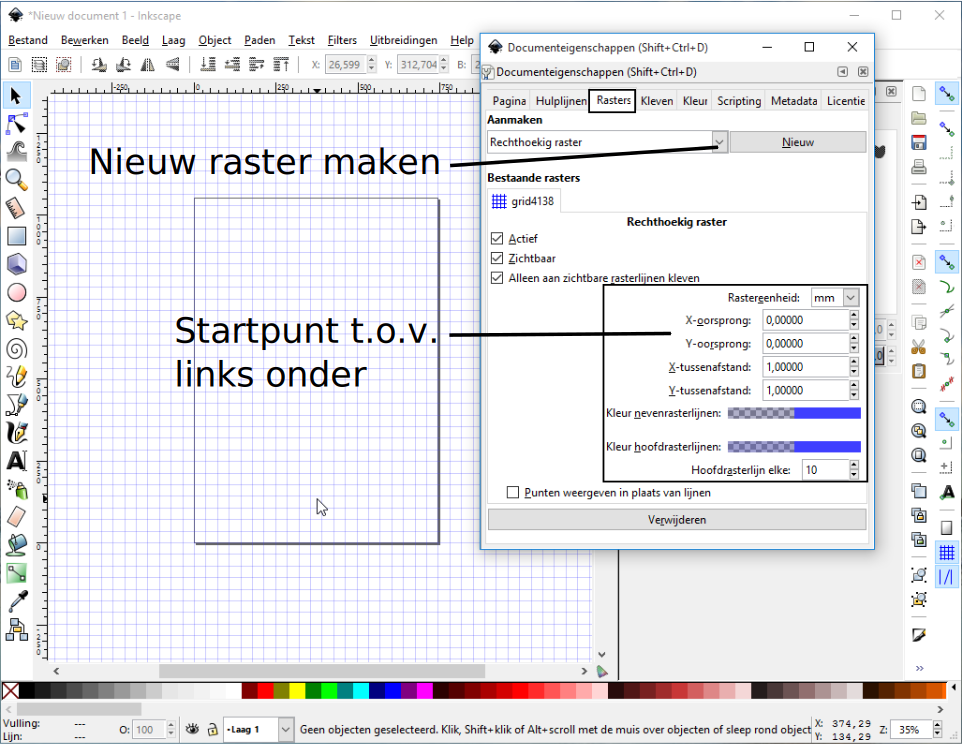
\includegraphics[height=0.8\textheight]{fig/inkscape_documenteigenschappen_rasters}
		\end{center}	
	\end{frame}
%%%%%%%%%%%%%%%%%%%%%%%%%%%%%%%%%%%%%%%%%%%%%%%%%%%%%%%%%%%%%%%%%%%%%%%%%%%%%%%%
	\begin{frame}
		\frametitle{Hulplijnen}
		\begin{columns}
				\begin{column}[T]{0.6\textwidth}
					\begin{itemize}
						\item Vanaf een lineaal slepen
						\item Slepen om te verplaatsen
						\item \textbf{Shift} + slepen om te draaien
						\item Dubbelklikken om meer gedetailleerde instellingen te wijzigen
					\end{itemize}
				\end{column}
				\begin{column}[T]{0.4\textwidth}
					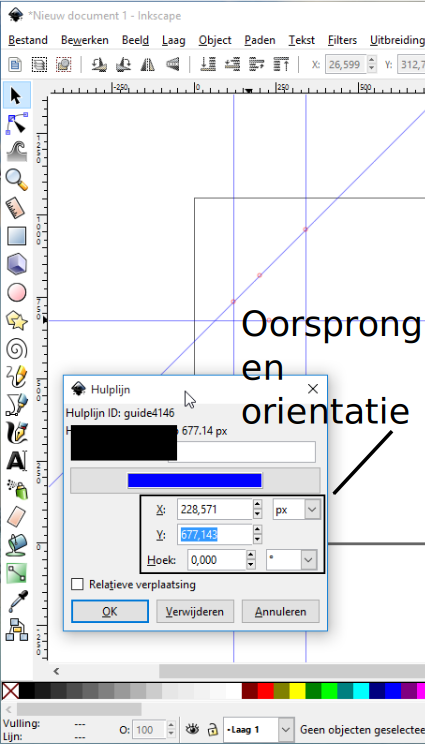
\includegraphics[height=0.8\textheight]{fig/inkscape_hulplijnen}
				\end{column}
			\end{columns}
	\end{frame}
%%%%%%%%%%%%%%%%%%%%%%%%%%%%%%%%%%%%%%%%%%%%%%%%%%%%%%%%%%%%%%%%%%%%%%%%%%%%%%%%
	\begin{frame}
		\frametitle{Kleven}
		\only<1>{
			\begin{columns}
				\begin{column}[T]{0.6\textwidth}
					\begin{itemize}
						\item Objecten, knooppunten en paden kunnen aan elkaar, rasters, hulplijnen,... kleven 
						\item Via kleven toolbar kiezen wat kleeft
					\end{itemize}
					\begin{itemize}
						\item Kleven aan knooppunten voor gesloten paden
						\item Kleven aan raster voor rechthoekige voorwerpen
						\item Kleven aan hulplijnen voor lijnen onder hoeken
					\end{itemize}
				\end{column}
				\begin{column}[T]{0.4\textwidth}
					\includegraphics[height=0.8\textheight]{fig/inkscape_kleven}
				\end{column}
			\end{columns}
		}
		\only<2>{
			\begin{center}
				
\includegraphics[height=0.8\textheight]{fig/raster_hulplijnen_paden}
			\end{center}
		}
	\end{frame}
%%%%%%%%%%%%%%%%%%%%%%%%%%%%%%%%%%%%%%%%%%%%%%%%%%%%%%%%%%%%%%%%%%%%%%%%%%%%%%%%		
	\section{Afbeeldingen importeren}
%%%%%%%%%%%%%%%%%%%%%%%%%%%%%%%%%%%%%%%%%%%%%%%%%%%%%%%%%%%%%%%%%%%%%%%%%%%%%%%%	
	\begin{frame}
		\frametitle{Importeren}
		\only<1>{
			\begin{columns}
				\begin{column}[T]{0.6\textwidth}
					\begin{itemize}
						\item Bitmaps importeren
					\end{itemize}
					\begin{itemize}
						\item Kleven aan knooppunten voor gesloten paden
						\item Kleven aan raster voor rechthoekige voorwerpen
						\item Kleven aan hulplijnen voor lijnen onder hoeken
					\end{itemize}
				\end{column}
				\begin{column}[T]{0.4\textwidth}
					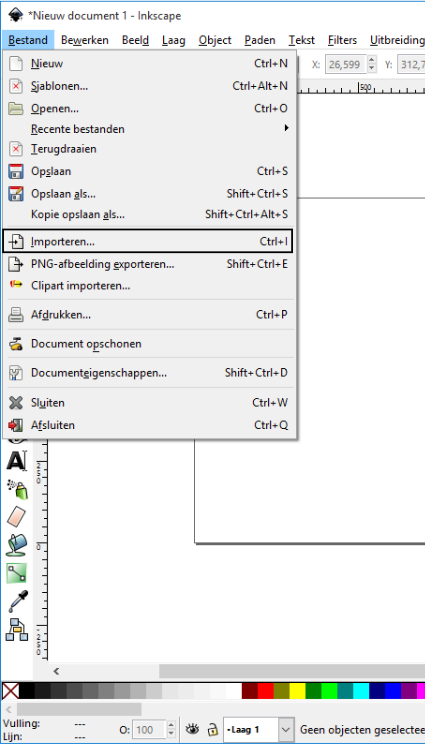
\includegraphics[height=0.8\textheight]{fig/inkscape_importeren}
				\end{column}
			\end{columns}
		}
		\only<2>{
			\begin{itemize}
				\item Bijsnijden van bitmaps (of andere figuren) moet via een omweg in inkscape
			\end{itemize}
			\begin{itemize}
				\item Maak een object in de vorm die je wil overhouden en zit dit over je figuur
				\item Selecteer beide objecten
				\item Ga naar \emph{Object $>$ Maskerpad $>$ Instellen}
			\end{itemize}
			
			\begin{center}
				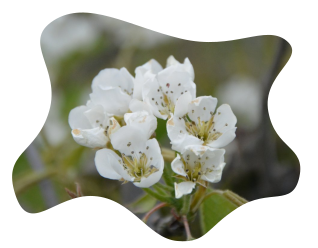
\includegraphics[height=0.5\textheight]{fig/bijsnijden}
			\end{center}
		}
	\end{frame}
	\begin{frame}
		\frametitle{Bitmap overtrekken}
		\only<1>{
			\begin{columns}
				\begin{column}[T]{0.6\textwidth}
					\begin{itemize}
						\item Bitmap figuur omzetten naar een Vector figuur
						\item Vaak veel handmatige correcties nodig
						\item Soms is de tekening handmatig omlijnen sneller
					\end{itemize}
					\begin{itemize}
						\item Verschillende algoritmes
						\item Helderheid: 1/3 (R+B+G) $<$ x \qquad vaak de beste keuze
						\item Randherkenning: lijnen met gelijke verandering in contrast
						\item Kleurmeting: lijnen met gelijke verandering in kleur
					\end{itemize}
				\end{column}
				\begin{column}[T]{0.4\textwidth}
					\includegraphics[height=0.8\textheight]{fig/inkscape_bitmap_overtrekken}
				\end{column}
			\end{columns}
		}
		\only<2>{
			\begin{center}
				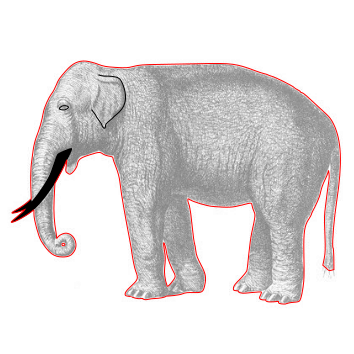
\includegraphics[height=0.8\textheight]{fig/bitmap_overtrekken}
			\end{center}
		}
	\end{frame}
%%%%%%%%%%%%%%%%%%%%%%%%%%%%%%%%%%%%%%%%%%%%%%%%%%%%%%%%%%%%%%%%%%%%%%%%%%%%%%%%	
	\section*{}
%%%%%%%%%%%%%%%%%%%%%%%%%%%%%%%%%%%%%%%%%%%%%%%%%%%%%%%%%%%%%%%%%%%%%%%%%%%%%%%%
	\begin{frame}
		\frametitle{Meer informatie}
		\begin{itemize}
			\item In inkscape \emph{Help $>$ Tutorials}
			\item https://inkscape.org/nl/learn/faq/
			\item https://inkscape.org/nl/learn/tutorials/
			\begin{itemize}
				\item verder klikken op Basic / Advanced / ...
				\item '.en.' in url vervangen door '.nl.' voor nederlands\\ \qquad .../x/tutorial-x.nl.html 
			\end{itemize}
		\end{itemize}
	\end{frame}
%%%%%%%%%%%%%%%%%%%%%%%%%%%%%%%%%%%%%%%%%%%%%%%%%%%%%%%%%%%%%%%%%%%%%%%%%%%%%%%%	
	\section*{}
%%%%%%%%%%%%%%%%%%%%%%%%%%%%%%%%%%%%%%%%%%%%%%%%%%%%%%%%%%%%%%%%%%%%%%%%%%%%%%%%
	\begin{frame}
		\footnotesize
		\vspace{4cm}
		\includegraphics[height=0.3cm]{fig/cc} \
		\includegraphics[height=0.3cm]{fig/by} \
		\includegraphics[height=0.3cm]{fig/sa}
		\quad \the\year\ Brecht Baeten
		\vspace{0.5cm}
		
    	Dit werk is gelicenseerd onder de licentie Creative Commons Naamsvermelding-GelijkDelen 4.0 Internationaal. Ga naar http://creativecommons.org/licenses/by-sa/4.0/ om een kopie van de licentie te kunnen lezen.
    	
    	\vspace{0.5cm}
    	De bron van dit document en alle tekeningen zijn beschikbaar op https://github.com/BrechtBa/inleiding-tot-inkscape
	\end{frame}	
	
\end{document}